% Document settings

% Common
\DocumentMetadata{pdfversion=1.7, pdfstandard=A-2u}
\documentclass[11pt,letterpaper]{article}
\usepackage{fancyhdr}
\usepackage[]{fncychap}
\usepackage{etoolbox} % patch stuff
\usepackage[margin=1in]{geometry}
\usepackage{multirow}
\usepackage{longtable,booktabs, array, threeparttable} % typesetting
\usepackage{bookmark}
\usepackage[acronym]{glossaries-extra}
\pagestyle{plain}
\usepackage{parskip, setspace}

% Plots and Color
\usepackage{graphicx}
\graphicspath{{images/}{drawings/}}
\usepackage[font=footnotesize,labelfont=bf]{caption}
\usepackage{xcolor,colorspace}
\usepackage{tcolorbox}
\usepackage{pgfplots}
\pgfplotsset{compat=newest}
\usepackage{epstopdf}
\usepackage[american voltages]{circuitikz}


% Math stuff
\usepackage{mathtools} % loads amsmath and fixes its bugs, empheq, etc
\usepackage{amssymb}
\usepackage{sympytex}
\usepackage{siunitx}
\sisetup{detect-all=true}   % ensure proper font weight
\sisetup{per-mode = repeated-symbol}    % ensure "/" unit delineator
\sisetup{range-phrase = {\text{~to~}}}  % SI range clarity (NIST 811 Ch7.7)
\DeclareMathSymbol{\varOmega}{\mathalpha}{operators}{"0A}   % upright omega for ohms
\providecommand*{\upOmega}{\varOmega}   % upright Ohms
\DeclareSIUnit{\sq}{\ensuremath{\Box}}    % sheet resistance
\DeclareSIUnit{\Siemens}{S}
\DeclareSIUnit{\torr}{Torr} % add torr to siunitix 3
\DeclareSIUnit\sig{\ensuremath{\sigma}}
\DeclareSIUnit\ppm{ppm}
\usepackage{xfrac}

% Font
\usepackage{fontspec}
\setmainfont{STIXTwoText}[
	Extension		= .otf,
	UprightFont		= *-Medium,
	BoldFont		= *-Bold.otf,
	ItalicFont		= *-MediumItalic.otf,
	BoldItalicFont 	= *-BoldItalic.otf
]
\usepackage[warnings-off={mathtools-colon,mathtools-overbracket},math-style=ISO]{unicode-math}
\setmathfont{STIXTwoMath-Regular.otf} % for symbols
% \usepackage{microtype}
% \UseMicrotypeSet[protrusion]{basicmath} % disable protrusion for tt fonts
\urlstyle{same}

\usepackage[normalem]{ulem} % Enable normal \ul underline
\usepackage{fancyvrb}

\RequirePackage[type={CC},modifier={by-nc-nd},version={4.0},lang={english}]{doclicense}

\usepackage{datetime2} % to satisfy the "\today" in \hypersetup
\DTMusemodule{english}{en-US}
\usepackage{hyperref}
\hypersetup{
    hyperindex=true,
    colorlinks=true,
	bookmarksnumbered,
    bookmarksopen=true,
    linkcolor=blue,
    filecolor=magenta,      
    urlcolor=cyan,
%%%%%%%%%%%%%%%% METADATA %%%%%%%%%%%%%%%%%%%%	
    pdftitle={EE726 Project 3},
	pdfsubject={4-Bit StrongARM Flash ADC},
    pdfauthor={Chris Biancone},
	pdfpublisher={Chris Biancone},
	pdfkeywords={rail-to-rail; StrongARM; flash ADC},
%%%%%%%%%%%%%%%%%%%%%%%%%%%%%%%%%%%%%%%%%%%%%%
	pdfproducer=luaLaTeX-1.17.0,
	pdfdate=\today,
	pdflang={en},pdfmetalang={en},
	pdflicenseurl={},
    % pdfpagemode=FullScreen,
}
\usepackage[nameinlink,capitalize]{cleveref}
% this is necessary for IEEEtranDOI.bst to work with hyperkinked DOIs
\newcommand*{\doi}{}
\makeatletter
\newcommand{\doi@}[1]{\href{https://doi.org/#1}{#1}}
\DeclareRobustCommand{\doi}{\hyper@normalise\doi@}
\makeatother

% % % % % % % % % % % Header footer
% % % % % % % % % % %EDIT THIS % % % % % % % % % % % % % % % % % % % %
\pagestyle{fancy}
\fancyhf{}
\lhead{Tech Memo:  Project 3}
\rhead{Chris Biancone}
\lfoot{EE726}
\cfoot{\today }
\rfoot{Page \thepage}
% % % % % % % % % % % % % % % % % % % % % % % % % % % % % % % % % % % % %

% Scale images if necessary, so that they will not overflow the page
% margins by default, and it is still possible to overwrite the defaults
% using explicit options in \includegraphics[width, height, ...]{}
%\setkeys{Gin}{width=\maxwidth,height=\maxheight,keepaspectratio}

% No paragraph indent
\setlength\parindent{0pt}

\begin{document}

\VerbatimFootnotes % allows verbatim text in footnotes

\numberwithin{equation}{subsection}
\numberwithin{figure}{subsection}

	\hspace{4.5in}
	
\includegraphics[width=2in,trim=0cm 0in 0in 0.0in,clip]{kgcoelogo2019horiz.eps}
\newline

\Huge\textbf{EEEE 726: Project 3 \\4-Bit StrongARM Flash ADC}\\

\Large
\textbf{From:} Chris Biancone \\
\textbf{To: } Dr. Mark Pude \\
\textbf{Date: } 04/02/2024 \\
\textbf{Subject: } Project 3\\
\vspace{0.5in}

\section*{Abstract}
\normalsize
The purpose of this project is to design a flash ADC incorporating the previously designed comparator. The RTR StrongARM-based comparator is refined to enhance the performance in this application. A 4-bit design is chosen based on the requirement for <\qty{25}{\dB} SQNR and each binary output is designed to drive a \qty{1}{\pF} capacitive load. This ADC has been tested to work in a rail-to-rail configuration with a reference voltage of \qty{2}{\V}, equal to the nominal supply voltage. In schematic-level simulations, a DNL of \qty{20.848}{mLSB}, INL of \qty{1.2009}{mLSB}, and propagation delay of \qty{2.7531}{\ns} are achieved at \(V_{LSB_{eff}}\) = \qty{133}{\mV}.

\section{Design}

The design of an \(N\)-bit flash ADC is geared toward brute-force comparison, where \(N-1\) comparators are biased at equal divisions within the range of the ADC reference volage, such that if the input \(V_{in}\) to the positive input of each ADC is higher than the reference at its negative input, the comparator trips its output high. While this topology requires high power due to the quescent draw of a reference gnerator for each comparator on top of the transient requirements of \(N-1\) comparators, it is robust and allows for very fast operation at 1 conversion per clock cycle.

\subsection{SQNR}

It is known that SQNR in an ADC system is a function of the bit depth of the ADC, since quantization noise is determined by the effective \(V_{LSB}\), shown in \cref{eq:sqnr}.

\begin{align}
    \mathrm{SQNR} &= 20\log\biggl(\frac{V_{in,rms}}{V_{Q,rms}}\biggr) \quad , \quad V_{Q,rms} \triangleq \frac{V_{LSB}}{\sqrt[]{12}}\\
    \mathrm{SQNR} &\approx 6.02\,N + \qty{1.76}{\dB}\label{eq:sqnr}
\end{align}

Thus, selecting \(N\) = 4 yields an SQNR = \qty{25.84}{\dB}, satisfying the design requirement of \qty{25}{\dB}. While this figure has little margin, SQNR is only a function of fundamental design aspects of the ADC as shown and will not vary with environmental conditions like noise or even reference voltage ranges.

\subsection{Top-Level}

A basic resistor ladder configuration was adopted for this ADC design to divide the reference voltage into individual references for each comparator. The resistors are arranged in an R : 2R $\cdots$ 2R : R configuration from top to bottom to divide the range into 2\textsuperscript{\emph{N}} ranges with 2\textsuperscript{\emph{N}}-1 voltages. Non-salicided \(p\textsuperscript{+}\) polysilicon resistors are chosen for their high sheet resistance to minimize layout area and relatively low temperature coefficient, and dummy resistors are enabled for manufacturing. \(R\) for these resistors is selected to be \qty{800}{\ohm}, which provides a balance of minimizing current draw from this stage and maintaining a reduced time constant when coupled with input capacitance of the comparators. This is necessary for kickback current noise that appears from the comparators -- which couples through the parasitic capacitance at the inputs -- to settle before their next sample. If the kickback voltage is significant compared to the voltage for each code, due to a high \(R\) value, this can result in glitches in the output. This can be characterized in the worst case by observing kickback at the middle of the ADC reference range, where the Thevenin equivalent resistance of the reference ladder is greatest and kickback will be worst. The downside to this configuration is that there is no way to correct for voltage variation that appears from variation in the global reference voltage, PVT variation, or process-induced mismatch; there is also no intrinsic kickback suppression, which is an important consideration when using dynamic comparators as proposed in this design. As such, a trade-off has to be struck between accuracy and preserving the low-power nature of the design provided by the comparator topology used\@. \cref{Fig:flash_sch} shows the full top-level schematic of the flash ADC, which consists mainly of the resistor network, comparators, and a thermometer-to-binary encoder for digitizing the comparator outputs. Since the comparators are dynamic and do not require current biasing, the provided \qty{10}{\uA} reference current is not used. More discussion is included later in this report on the instances shown at the top left of \cref{Fig:flash_sch}.

\begin{figure}[t!]
		\centering
		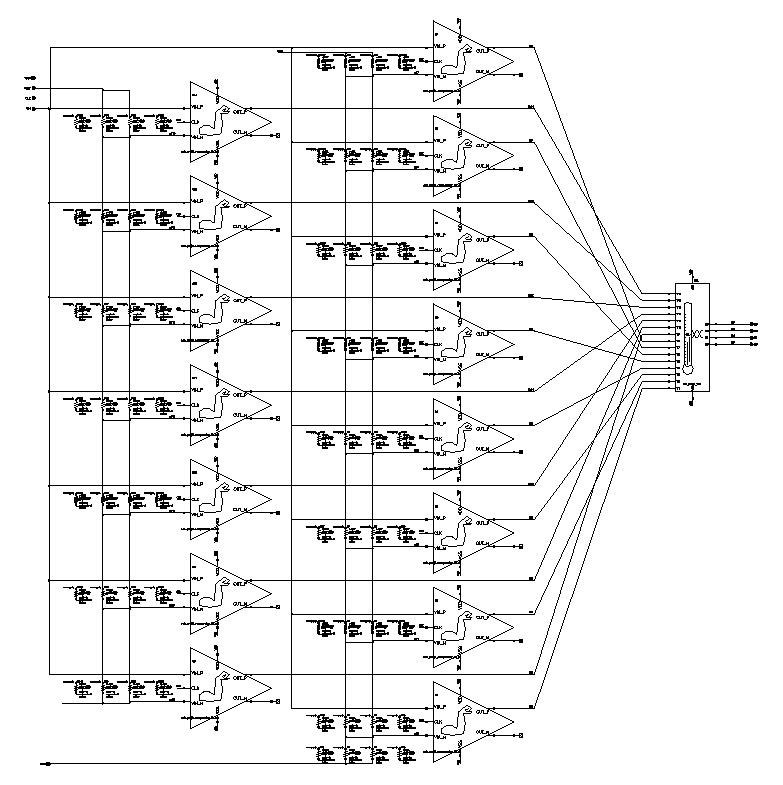
\includegraphics[width=4in]{flash.eps}
		\caption{Top-level schematic of the flash ADC.}\label{Fig:flash_sch}
\end{figure}

\subsection{Comparator}

The StrongARM comparator employed in this ADC is designed to process rail-to-rail common mode signals, allowing the same exact comparator design to be used for every position. This avoids any mismatch in input capacitance throughout the range and should contribute toward gain linearity across the common mode range. The schematic design of this comparator has remained unchanged from Project 2, as shown in \cref{Fig:comaprator_v2_sch}, but the layout has been reworked to simplify routing with the intent of reduced parasitics and decreased layout area, detailed later in this report.

\begin{figure}[t!]
    \centering
    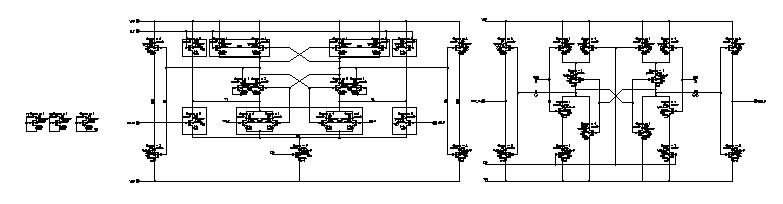
\includegraphics[width=\textwidth]{comp_full.eps}
    \caption{Schematic of the RTR StrongARM comparator as employed in this flash ADC design and its associated SR latch.}\label{Fig:comaprator_v2_sch}
\end{figure}

The performance of the revised layout was verified through extracted simulations, and was found to work to the previous design specifications up to a speed of about \qty{1.1}{\GHz}. Above this speed, hysteresis began to rise to values greater than would have been acceptable for the ADC, as any amount of hysteresis contributes to nonlinearity of the flash ADC due to differences in rising and falling trip voltages. While not simulated with noise sources, less than \qty{15}{\mV} of hysteresis is designed into the comparator in extracted simulations at the provided cock speed of \qty{12}{\MHz}, providing a balance between linearity and stability with a noisy input source. Further reduction of hysteresis and increase of speed was found to be difficult due to the limits imposed by the use of the \qty{2}{\V} device in the gpdk\_045, which have a minimum length of \qty{180}{\nm} and finger width of \qty{320}{\nm}. The performance is detailed in \cref{tab:comp_perf}.

\begin{table}[]
    \centering
    \begin{tabular}{ccc}
    \toprule
        Parameter & Units & Nominal \\
    \midrule
        Hysteresis & mV & 14.64 \\
        Prop. Delay (\qty{1}{\pF}) & ns & 1.5778 \\
        Prop. Delay (\qty{1}{\fF}) & ps & 414.07 \\
        DC Current & nA & 1.2868 \\
        W/decision & pW & 1.067 \\
        Layout Area & \(\qty{}{\um^2}\) & 119.79 \\
    \bottomrule
        
    \end{tabular}
    \caption{Comparator performance with extracted parasitics from layout.}\label{tab:comp_perf}
\end{table}

\subsubsection{Threshold Modification}

Incidentally through some simulations, it was found that varying the input device sizes for this comparator design yielded control over the trip voltage, and this could be exploited to achieve adjustment over the entire supply range. With this in mind, tuning different comparator design was explored as a possibility to create a flash ADC without the use of a resistor biasing string, creating an ultra low power and layout area design. Simulations were run to determine the trip voltage for some initial coarse device sizing, with the intent of producing an experimental curve to further refine the choice of sizes. While sizing to process the entire lower half of the input range was achieved, the relationship to trip voltage was found to be very nonlinear, which would likely negatively impact mismatch results and could have other implications. This method would have also presented different input capacitances at each level of the input range, which may introduce nonlinearity as well. While this idea may still benefit from some future work, the time dedication did not fit within the scope of this project and the previously mentioned reference generation scheme was used.

\subsection{Encoder}

Some form of encoder subsystem is necessary in the flash ADC to translate the ``thermometer''-coded output of the 15 comparators into 4-bit binary. Various methods have been explored in industry and literature, including Wallace tree, Fat-tree, ROM, and MUX based designs. Other algorithms sometimes perform a conversion to gray code before binary to provide robustness against ``bubble errors'' caused by a comparator improperly evaluating as 0 below one that has evaluated as 1. Additional logic to perform this correction can also be added onto the other encoding methods as well. A MUX-based ``priority'' encoder design based on~\cite{Sall2007} is used for its low-power operation and high speed at the cost of high device count, shown in \cref{Fig:encoder}. No bubble correction was implemented in this design, as the low bit-depth of this ADC compared with the resolving capability of the comparators used should additional power savings and reduction in the number of required devices is provided through the use of transmission gate-based MUXs shown in \cref{Fig:tgmux2}, which use half the number of devices as active CMOS multiplexers. To provide delay time correction for the MSBs of the encoder, additional self-selected MUXs are added to each to match the critical path for the LSB\@. This minimizes glitches due to different bit arrival times and the self-selecting MUXs should add enough consecutive delay to allow the LSB to arrive first, minimizing the magnitude if a glitch occurs. The additional devices needed to provide this functionality are not viewed as a significant penalty due to the device savings from using TG MUXs. 

\begin{figure}[htbp!]
    \centering
    \includegraphics[width=4in]{encoder.eps}
    \caption{Schematic view of encoder design.}\label{Fig:encoder}
\end{figure}

\begin{figure}[htbp!]
    \centering
    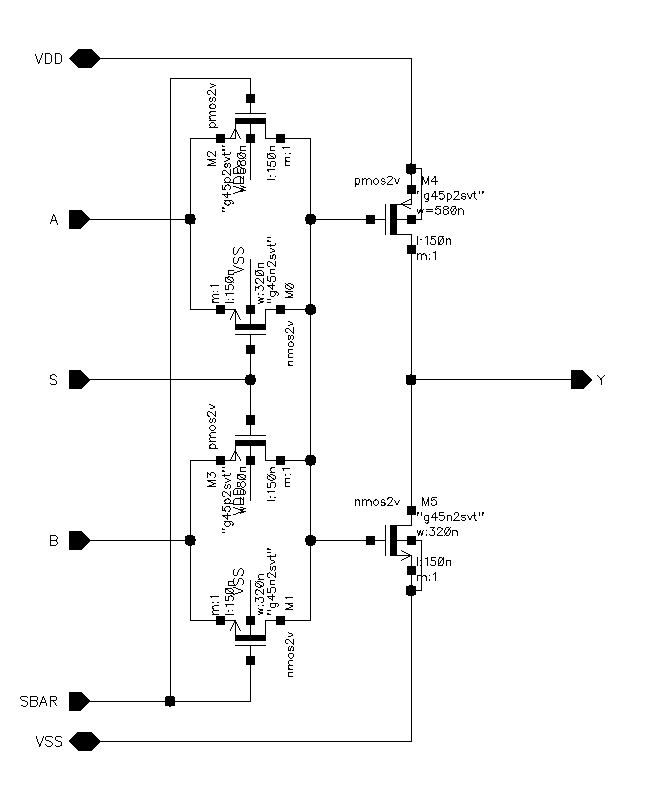
\includegraphics[width=3in]{tgmux2.eps}
    \caption{Schematic of transmission-gate based MUX that provides the functionality of the proposed encoder design. The outputs are inverted for logic purposes and increased drive strength.}\label{Fig:tgmux2}
\end{figure}

\begin{figure}[htbp!]
    \centering
    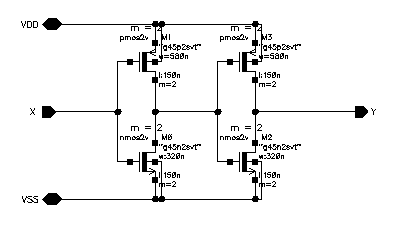
\includegraphics[width=4in]{buf.eps}
    \caption{Schematic of buffer highlighting device sizes, which are also used in the inverter design.}\label{Fig:buf}
\end{figure}


\section{Schematic Level Simulations}

Schematic simulations were performed over PVT corners and monte carlo analysis. The process corners used were tt, ss, sf, fs, and ff, temperatures of 0, 27, 40, and \qty{85}{\degree\C}, and supply voltages of 1.8, 2.0, and \qty{2.2}{\V}. The schematic was captured and simulated using C\=adence Virtuoso. 

\subsection{INL and DNL Testbench}

A simple testbench schematic was set up for the flash ADC as shown in \cref{fig:tb-sch}. The local ground for this design is decoupled from the global ground using a \qty{0}{\V} source, and currently a VCVS is used to increase the given reference voltage of \qty{1}{\V} up to \qty{2}{\V} for testing rail-to-rail operation. In a full system, a reference voltage at the power supply would likely need to be supplied by an LDO and possibly assisted by a charge pump. The supplied \qty{12}{\MHz} clock is realized by a pulse source with 5\% rise and fall times, and the input triangle ramp is supplied by a piecewise-linear source. 

For the voltage reference, a \qty{1}{\V} DC supply is used as a given refrence per design specifications. To enable testing at a reference of \qty{2}{\V} to evaluate rail-to-rail operation, a \emph{vcvs} was used to step up the voltage. This was done under the assumption that a stable reference is being provided 

Each output bit from the encoder drives a \qty{1}{\pF} load as specified, and are also sent into an ideal 8-bit DAC provided by the \emph{ahdlLib}. This DAC is intended to translate the binary ADC output into a stepped ramp output for comparison with the ideal stepped ramp output with idealized trip voltages. Once normalized for any gain and offset error using the first and last transitions to find a \(V_{LSB_{eff}}\), the difference in code widths for the output of the ADC compared to the ideal version defined by variables in teh ADE Assembler Environment allows for quantification of differential nonlinearity (DNL). The summation of these differences across the range provides the integral nonlinearity (INL). This simulation setup provides a similar feel to evaluating these specifications for a continuous time comparator, but instead of the precision being defined by the number of voltage steps per digital code, it is defined by the number of clock cycles per code. Therefore, the testbench setups were completely parametrized around this figure to allow for quick changes if necessary.

\begin{figure}[!t]
    \centering
    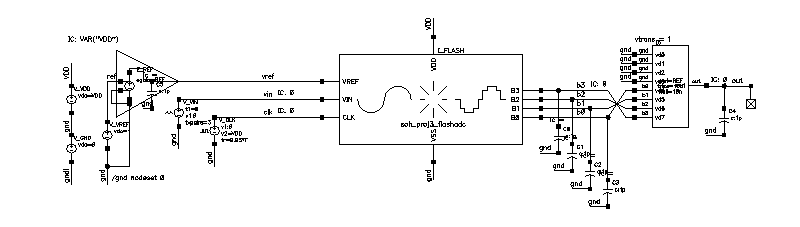
\includegraphics[width=6in]{flash_tb.eps}
    \caption{Testbench setup used for INL and DNL analysis.}\label{fig:tb-sch}
\end{figure}

The achieved results for INL and DNL at typical corner are shown in \cref{fig:inldnl}. \(V_{LSB_{eff}}\) was calculated to be \qty{133}{\mV}.

\begin{figure}[htbp!]
    \centering
    \includegraphics[width=4in]{INL_DNL_TYP_old.png}
    \caption{INL and DNL results at typical.}\label{fig:prop-plot}
\end{figure}

\subsection{Propagation Delay Testbench}

To analyze propagation delay, the same testbench setup was used but with a modified PWL input to step nearly instantaneously right before each evaluation at the clock rise. This was intended to have all the comparators slam high or low at once, and the last output bit to fall into place was measured for propagation delay. The outputs were evaluated at both rising and falling inputs, and the maximum time for any of the bits to transition was measure, giving a worst-case delay figure. The results are shown in \cref{prop}.

\begin{figure}[htbp!]
    \centering
    \includegraphics[width=4in]{TP_TYP_old.png}
    \caption{Propagation delay results at typical.}\label{fig:prop}
\end{figure}


\subsection{Issues Faced}

Simulating the performance of this ADC design proved to be a significant challenge from both the standpoint of computational intensity and unexpected inconsistencies from one run to the next. Testing was initially performed using only a single defined TYP corner, due to the simulation time needed to see the effect of changes made to the design. To aid the solutions, initial conditions and node-set values were provided for appropriate top-level nodes for transient and DC simulations to use respectively. Pivoting was enabled for DC simulations using the gear2 method. Initially, Spectre APS was used with ++aps enabled and conservative error preset for both testbenches, and then an explicit +mt=8 was added. For the propagation delay analysis, Sometime during testing, the comparator outputs all began solving improperly, rising at the beginning of the simulation before the first clock edge. It was found that disabling ++aps resolved this issue. (Further discussion with classmates provided insight that it may be beneficial to enable options in Spectre to explicitly prevent it from using prior run data to inform the solution of the current run, which may have effectively been what happened by changing the simulator settings here.) Using Spectre X with AX preset, AX parasitic optimization, and 8 threads decreased the INL/DNL testbench simulation time from \~4:\qty{15}{min} to \~2:\qty{30}{min} with no apparent change in accuracy, so this was implemented for the final results. For the INL/DNL testbench, MS simulation was also enabled with the encoder selected as a digital instance and the comparators and clock buffer selected as analog instances; the propagation delay testbench remained with MS simulation disabled. While the 21.3 version of Spectre used offers massively parallel GPU simulation capability, the license available does not have access to this feature.

Monte carlo simulations also proved to be a sticking point, and at the point of writing it is still unclear if the results obtained for DNL in these simulations are accurate, both due to the low LSB precision and number of monte carlo points required to complete any simulations before the submission was due, and the large disparity in yield with the comparator results, which makes up the bulk of the devices in the ADC\@.

The stated simulation times are for 10 clock cycles per digital code, giving a maximum evaluation precision of \qty{0.1}{LSB}. To truly quantify the performance of the ADC itself, a precision of \qty{1}{mLSB} was desired, but this did increase the simulation time for each test tenfold. As such, a balance between quantifying performance and quantifying the design's ability to meet specifications had to be struck, and the accuracy for the results will be noted. 

At some point during testing, tests were rerun after reopening Cadence and the INL/DNL testbench results were much worse than before. DNL has increased from around \qty{20}{mLSB} to well over \qty{1}{LSB} and INL increased from around \qty{8}{mLSB} to around \qty{100}{mLSB}. At this point, \qty{13}{\kilo\ohm} resistors were being used for power savings. It is believed that something changed in the evaluation of the kickback voltage presented at each comparator's reference input, as it was eventually found that decreasing the resistor ladder values provided small improvements to INL and DNL\@; this change would have reduced the discharge time constant at the nodes through the overall reduced Thevenin equivalent resistance, providing less of a severe impact on the transition voltages. Something of note is that this was most severely affecting the bottom of the range, whereas the worst reference disturbance would be expected to be in the middle where the Thevenin resistance would be highest. While the root cause of the new disappointing results could not be determined, further reduction of the resistor values did improve INL and DNL values to acceptable levels. 

To further reduce nonlinearity to meet spec by a reduction of kickback, a quasi-adiabatic drive system was constructed. This involves simply adding an RC time constant to the local clock line to reduce the slew rate of the clock signal; a more slowly ramping clock reduces kickback since the current noise coupled back to the comparator input is related to the discharge rate of the StrongARM's internal nodes, as shown in \cref{eq:kickback}, where \(dV_A\) is the time-varying voltage at the sources of the input transistors and \(dV_P\) is the time-varying voltage at the drains~\cite{Yousefirad2021}. 

\begin{equation}
    I_{kickback} = -\biggl(\frac{2}{3}W\,L\,C_{ox} + C_{GS_{tot}}\frac{dV_A(t)}{dt} - C_{GS_{tot}\frac{dV_P(t)}{dt}}\biggr)\label{eq:kickback}
\end{equation}

\noindent Also shown by this relationship, kickback is increased in the comparators used due to both the large minimum size of the \qty{2}{\V} transistors used and the inclusion of parallel NMOS and PMOS input devices for RTR operation. 

The quasi-adiabatic drive is implemented in this design by employing a transmission gate to provide separately tunable effective resistance for both clock edges, which couples with the input capacitance of the comparators to round off the rising and falling edges of the clock. Since kickback noise generated on the falling clock edge does not impact the comparator evaluation, as long as the fluctuation does not last until the rising edge of the clock, a smaller NNOS device is used, while \qty{640}{\nm} length PMOS devices are used to round the clock more. A local clock buffer is provided to decouple the transmission gate from the ideal clock source used, and is beneficial to have in the final ADC layout; these are shown in the top left of \cref{Fig:flash_sch}. While the use of metal resistors would provide better uniformity across corners, the transmission gate structure offers beneficial dynamic response for this circuit, and additional variation robustness can be provided by increasing the size of these devices. Another important consideration is that this approach makes the comparator decision more and more asynchronous with the system clock as more smoothing is designed, causing an effective increase in propagation delay.

Some other ideas were investigated to reduce the kickback voltage, such as increasing the capacitance at each of the reference steps and even instantiating an inductor on the reference line for the middle comparator, to function as a choke where the kickback is greatest. While the capacitances were not enough to provide significant benefit, the inductor performed surprisingly well initial simulations, bringing INL and DNL below measurement precision instantly. Across corners, however, a sinusoidal-shaped output plot in the codes surrounding the middle reference began to appear, suggesting that the choke began to act more like a tuning fork. Combined with the comically large size of the inductor pcells and the added manufacturing cost of the top metal layers needed, this solution provided little benefit for real implementation.

\subsection{Schematic Level Results}

The ADC design passed the \qty{30}{\ps} propagation delay and \qty{1}{LSB} INL specifications with flying colors across corners, and passed the \qty{500}{mLSB} DNL in 50/60 corners for the given \qty{1}{\V} reference. This is most likely due to some more kickback suppression needed to account for the worst corners as these failures all occur at low supply voltages, with the worst DNL occurring always in the middle of the range. A solution was not able to be implemented at the time of writing due to the issues faced and time needed to wait for the simulations to run. The results captured in \cref{tab:corners_sch} are obtained with 10 clocks per code giving a precision of \qty{100}{mLSB}, and should not be taken as a quantitative maximum performance evaluation of the ADC\@. A simulation was run at the typical corner with 1000 clocks per code, to hopefully get a sense of the true performance of the ADC, which may be cautiously extrapolated across the corner results; this is presented in \cref{tab:typ_sch}.

\begin{table}[]
    \centering
    \begin{tabular}{ccccc}
    \toprule
        Parameter & Units & Max & Nominal & Min \\
    \midrule
        DNL & mLSB & 4821.7 & 153.8 & 60.21 \\
        INL & mLSB & 16.009 & 9.2979 & 2.3985 \\
        Max Prop. Delay & ns & 13.253 & 7.4131 & 5.7102 \\
        Timing difference & ps & 213.44 & 148.72 & 18.045 \\
        Reference DC Current & \qty{}{\uA} & 192.95 & 148.72 & 123.55 \\
        Max Transient Current & mA & 15.358 & 8.4772 & 3.502 \\
        W/conversion & pW & 101.38 & 63.452 & 37.654 \\
    \bottomrule
        
    \end{tabular}
    \caption{Flash ADC performance results across PVT corners, with a precision of \qty{10}{mLSB} for DNL and INL measurements.}\label{tab:corners_sch}
\end{table}

\begin{table}[]
    \centering
    \begin{tabular}{ccccc}
    \toprule
        Parameter & Units & Nominal \\
    \midrule
        DNL & mLSB & 115.61 \\
        INL & mLSB & 7.2199 \\
        \(\mathrm{V_{LSB_{eff}}}\) & mV & 66.4 \\
    \bottomrule
        
    \end{tabular}
    \caption{Flash ADC DNL \& INL results at the typical corner, with a precision of \qty{1}{mLSB}.}\label{tab:typ_sch}
\end{table}

Interestingly, the worst codes for DNL in this simulation are at the extents of the reference range, with single-digit mLSB DNL seen in the middle of the range.

Monte carlo simulations for this design are unknown to be properly simulated. Propagation delay resulted in a 100\% yield over 3-\(\sigma\) variation, but the histogram shown in \cref{fig:tp_mc} has a very unusual distribution characteristic. Nonlinearity testing had to be conducted with fewer points, and INL testing produced 100\% yield with a more normal histogram shown in \cref{fig:inl_mc}. DNL measuremnts produced no usable results with only quantities in aLSB or around 12-\qty{14}{LSB} given. This gives pause as to the validity of the INL measurements as well, due to its reliance on properly evaluated DNL. 

\begin{figure}[ht!]
    \centering
    \includegraphics[width=4in]{tp_mc.eps}
    \caption{Propagation delay monte carlo histogram.}\label{fig:tp_mc}
\end{figure}

\begin{figure}[ht!]
    \centering
    \includegraphics[width=4in]{inl_mc.eps}
    \caption{Integral nonlinearity monte carlo histogram.}\label{fig:inl_mc}
\end{figure}

A sensitivity analysis was run over the course of a day to see if a trend could be found in what contributed to the spread of DNL measurements, but the results from this were unclear as well. Shown in \cref{fig:sens_dnl}, no device had considerable contribution to DNL variation in the entire design. This is somewhat expected due to the sheer number of devices in the design; however, no pattern is observed in the top contributors either. It was expected to see a consistent device within all of the comparators contributing mostly to DNL variation, but this was very much not the case. Further investigation into this issue is needed to quantify the design's performance under mismatch.

\begin{figure}[ht!]
    \centering
    \includegraphics[width=\textwidth]{sens_inl.png}
    \caption{Sensitivty analysis results ordered in highest contribution to DNL variation.}\label{fig:sens_dnl}
\end{figure}

\section{Layout}

The first layout completed for this design was the comparator shown in \cref{fig:comp_v2_layout}, since this had to be modified and then verified as it is the center of the ADC operation. Moving the large PMOS switches to the center of this design now line up their drain routing with the input transistors, which greatly simplifies much of the overall routing of this design. This also further increases the symmetry of the overall layout, and should enhance the matching of the input transistors as well. Cross-coupled devices M5 and M6, and the other PMOS switches are now also split and common-centroided alongside the input devices. The majority of the internal guard rings are removed, to allow for tighter spacing between the NMOS and PMOS devices. Metal 4 is used for connections external to the comparator, which allows for routing a few more long-range connections on Metal 3 to reduce capacitance to other signals.

\begin{figure}[ht!]
    \centering
    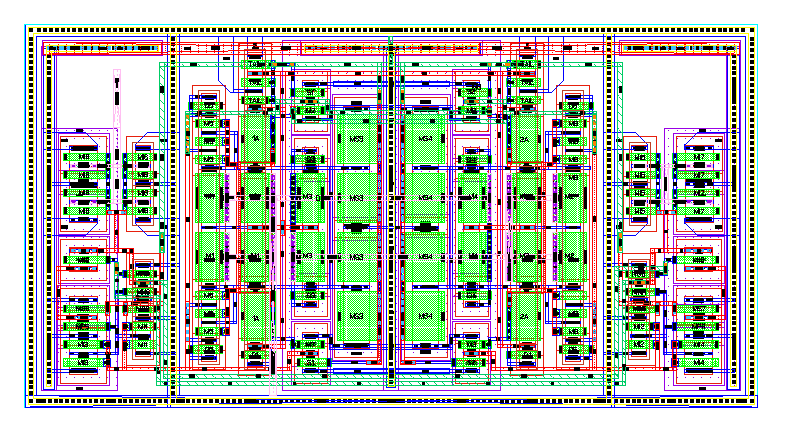
\includegraphics[width=\textwidth]{comp_v2_layout.eps}
    \caption{Comparator layout, version 2.}\label{fig:comp_v2_layout}
\end{figure}

After this, the low-level digital blocks needed were laid out, with a design that enables them to be instantiated as a long row in the upper level layout to allow for simpler power rail routing, shown in \cref{fig:mux2_tg_layout}.

\begin{figure}[ht!]
    \centering
    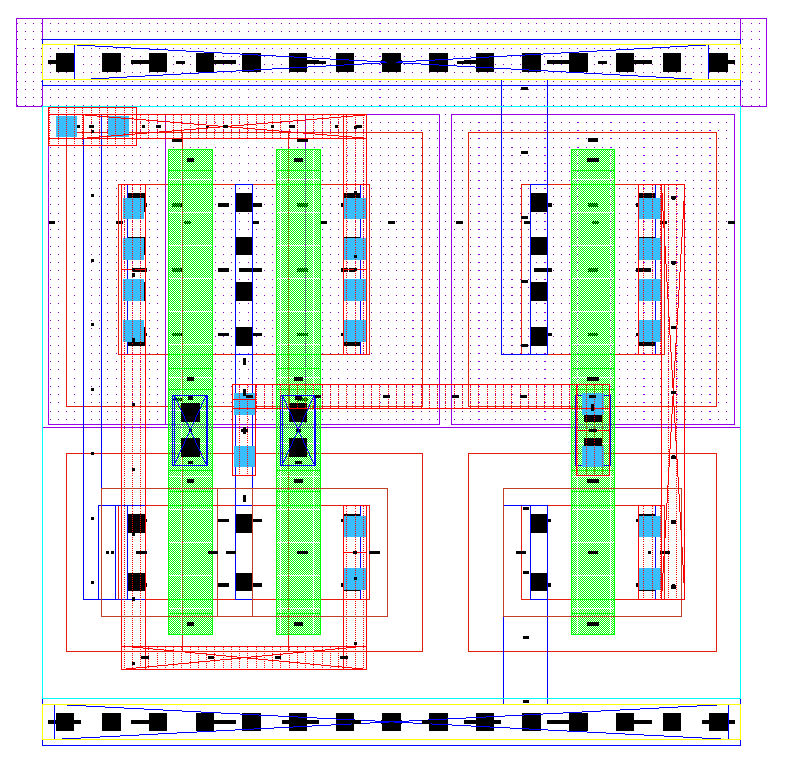
\includegraphics[width=4in]{mux2_tg_layout.eps}
    \caption{Transmission gate MUX2 with inverter layout.}\label{fig:mux2_tg_layout}
\end{figure}

With the MUXs and inverters completed, the full layout of the encoder was completed. The design takes advantage of the rail configuration of the digital blocks, and is completed in two horizontal rows, with power rails on the sides and in the middle. The auto-routing feature within Cadence Virtuoso was employed to route this block for time considerations, since the digital circuitry is more immune to routing decisions made by an algorithm such as this. Routing was allowed on metals 2 to 4 with 2 and 3 preferred, and was done using the ASIC preset. The results are shown in \cref{fig:layout_t2b}.

\begin{figure}[ht!]
    \centering
    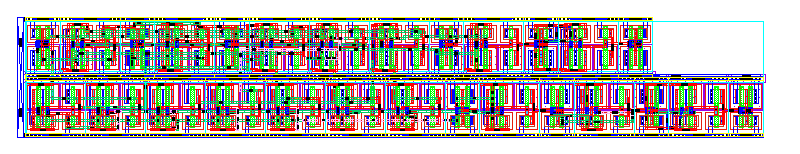
\includegraphics[width=\textwidth]{t2b_layout.eps}
    \caption{Thermometer to binary encoder layout.}\label{fig:layout_t2b}
\end{figure}

The overall comparator layout began with floor plan to have two columns of comparators with resistors located in the middle, to ensure better matching between the resistors which is critical for the flash topology. Due to the short nature of the encoder block, it could be placed within the space left due to having 15 comparators, and the adiabatic drive devices could find a home in the middle.

Routing of the full ADC was done by hand to ensure symmetry, and once all signals were routed the clock line to all of the comparators was auto-routed using the same settings as before. VDD and VSS lines to the comparators were overlapped as much as possible on metals 1 and 2 to provide as much capacitance as could be easily obtained. The final result is shown in \cref{fig:flash-layout}. The final ADC layout size is \qty{59.25}{\um} by \qty{68.265}{\um} for a total area of \qty{4044}{\um\squared}. Both DRV and LVS evaluated clean on this layout.

\begin{figure}[ht!]
    \centering
    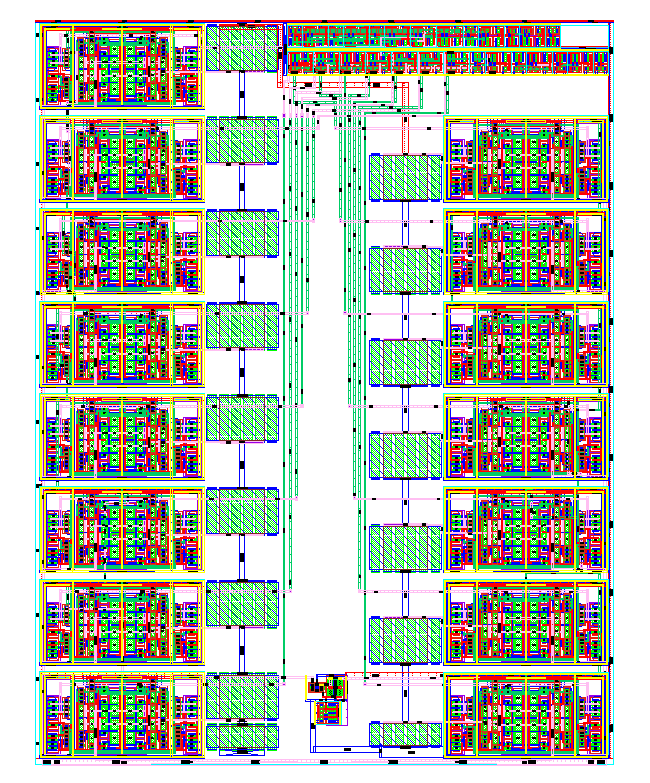
\includegraphics[width=\textwidth]{flash_layout.eps}
    \caption{Full flash ADC layout.}\label{fig:flash-layout}
\end{figure}

\section{Extracted Results}

At the time of writing, extracted simulations have not been run across corners due to the simulation time required and a desire to iron out more of the simulation tool kinks before doing so.

\section{Conclusion}

A lot has been learned through the completion of this project, both about the creation of a flash ADC and about simulation and verification of mixed signal circuit designs. The simulation tools have definitely shown their learning curve, and a lot of new approaches had to be explored due to this non-traditional design with dynamic comparators. The ADC design itself was mostly successful, and there is a clear path to be taken to resolve the operation at failed PVT corners. The monte carlo results are less clear, and more investigation is needed to see if the results are valid or what can be done to improve their evaluation.

\newpage

\bibliographystyle{bib/IEEEtranDOI}
\bibliography{bib/main.bib}

\newpage
\section*{Appendix}

\begin{figure}[ht!]
    \centering
    \includegraphics[width=4in]{drc.png}
    \caption{DRC results.}\label{fig:drc}
\end{figure}

\begin{figure}[ht!]
    \centering
    \includegraphics[width=4in]{lvs.png}
    \caption{The Holy Grail.}\label{fig:lvs}
\end{figure}

\end{document}